\chapter{Návrh}\label{chap:design}
Tato kapitola se bude zabývat návrhem sestavy technologií které se budou využívat pro realizaci API.

\section{Model vývoje}\label{sec:development_model}
Jako model vývoje byl použit typický vodopádový model \figureref{fig:waterfall}. Není to realistický model ale je základem pro většinu ostatních modelů a je velice jednoduchý. Používá se primárně v situacích kdy definice projektu je jasná a je jasný cíl, kdy je dost času pro vývoj a je málo místa pro chyby.

Vlastnosti tohoto modelu jsou \textbf{sekvenční přístup}, neboli dokud není hotová první část tak se nepřechází na další. Další z vlastností je \textbf{řízena dokumentací}, neboli během ostatních fází se nemusí přemýšlet jak co má fungovat a stačí to jen napsat. \textbf{Kontrola kvality} je při tomto modelu důležitá, neboť chyby které by se mohli vyskytnout v prvnotních fázích vývoje se mohou nepříjemně projevit a vývoj zkomplikovat. s tím se pojí i \textbf{přísné plánování}

Tímto modelem jsme se snažili řídit ale i přes dobré rozmyšlení si návrhů se muselo v průběhu pár drobností upravovat. 

\begin{figure}[!ht]
    \centering
    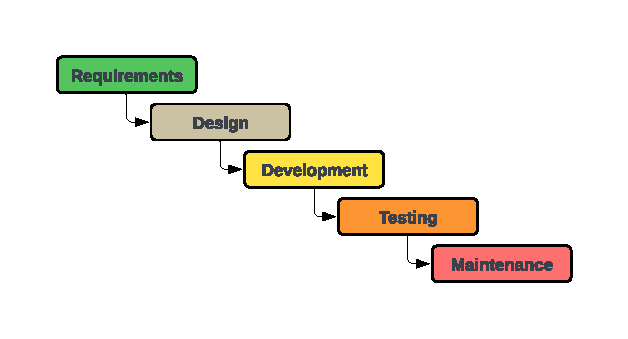
\includegraphics[width=0.8\textwidth]{figures/impl/API Implementation - waterfall model.pdf}
    \caption{Vodopádový model vývoje}\label{fig:waterfall}
\end{figure}

Ve fázi \textbf{požadavků} probíhali nápady jak samotná hra bude fungovat, jaké mechaniky použijeme a jak by šli implementovat. V této fázi vystačí pouze dokument s nápady a požadavky. Taktéž si všichni ujasnili a shodli se jaké herní mechaniky budou použity a za jakých okolností. 

Ve druhé fázi \textbf{návrhu} se navrhují upřesňující diagramy, návrh architektury a návrhy UI. V našem případě byly přesněji rozvrženy jednotlivé mechaniky a co se od nich očekává. Zároveň spoustu návrhu za nás řeší vybraný framework pro tvorbu API a fakt že se bude jednat o RESTful API. 

Fáze \textbf{vývoje} zahrnuje implementaci návrhů a vytvoření funkčního programu. V této fázi se taktéž využívají unit testy zda jednotlivé komponenty jsou funkční. 

A poslední fáze \textbf{testování} a \textbf{údržba} se stará o to aby program byl bez chyb a vše fungovalo jak má jakožto celek. Po tom co byl projekt otestován a vše je funkční tak jde do produkčního prostředí a už se pouze udržuje což zahrnuje opravování drobných chyb které nebyly odhaleny v testování.

\section{Spolupráce}\label{sec:collaboration}
Jak už několikrát bylo naznačeno, tato práce se vytvářela v týmu a každý měl na starosti jinou hlavní komponentu.
\begin{itemize}[itemsep=0pt,parsep=0pt]
    \item \textbf{Herní systém} -- Barbora Kovalská
    \item \textbf{Backoffice} -- Pavel Mikula
    \item \textbf{Frontend} -- Mirek Osoba
    \item \textbf{API} -- Martin Korotwitschka
\end{itemize}

Ovšem některé komponenty se musely přidat protože byly potřeba pro samotné zprovoznění hry jakožto celku, takže zvlášť na nich pracovalo více členů týmu. V ranních fázích vývoje bylo taktéž běžné že více členů více či méně se podílelo i na ostatních úkonech. 

Komunikace probíhala zvlášť v prvotních fázích vývoje za pomocí nástroje Github Issues a později, když už kostra projektu byla funkční, tak stačila interní komunikace.  
\subsection{Rozdělení práce}\label{sec:collaboration:job_distribution}
Jak lze vidět na \figureref{fig:job_distribution} tak každý člen týmu měl na starosti svou část projektu. Toto rozdělení vycházelo především ze zadání prací. 

\begin{figure}[h]
    \centering
    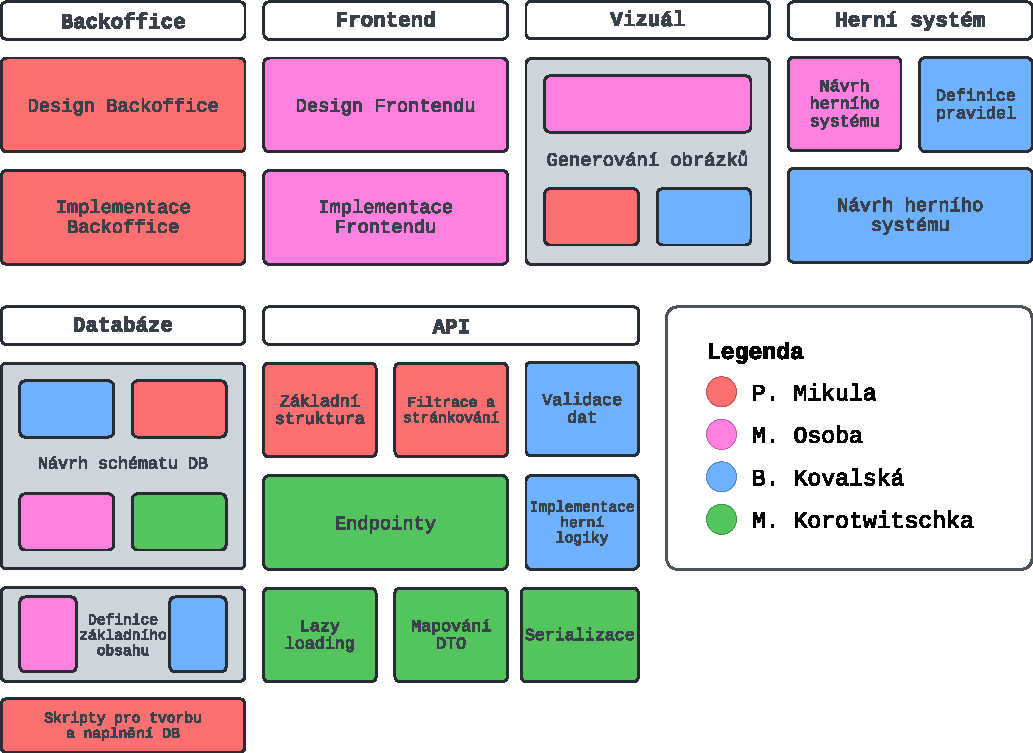
\includegraphics[width=\textwidth]{../../shared/diagrams/blocks.pdf}
    \caption{Rozložení práce v týmu}
    \label{fig:job_distribution}
\end{figure}

Pro přehlednost a pro verzování kódu byla vytvořena organizace na Githubu \figureref{fig:gitOrg}, kde se vytvořili samostatné repozitáře pro každou část celého projektu. Taktéž se zde vedly \textit{Issues} které zvlášť v prvotních fázích ulehčovali vývoj a komunikaci. 

\begin{figure}[H]
    \centering
    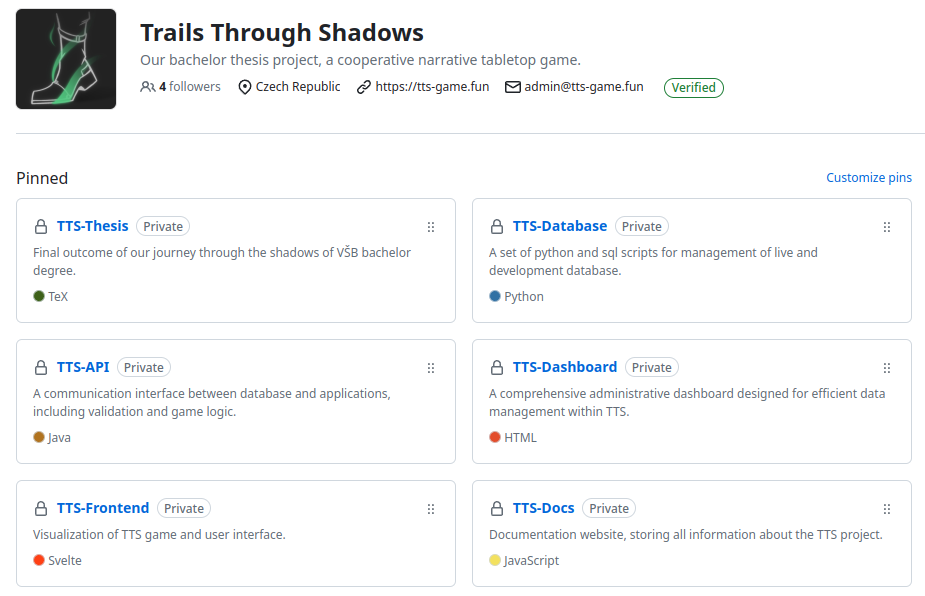
\includegraphics[width=\textwidth]{../../shared/figures/gitOrg.png}
    \caption{Organizace \textit{Trails Through Shadows} na Githubu}
    \label{fig:gitOrg}
\end{figure}


Verzovací systém byl zvlášť potřeba v případě API, na kterém pracovali primárně dva členové týmu. Tím pádem bylo využíváno tzv. větví pro iimplementování rozličných funkcionalit. Ovšem když ještě nebyla kostra API tak takovéto rozdělování na větve není tak účinné a často se museli řešit konflikty. 

Poté co byla vytvořena kostra API se začali řádně využívat větvě a jejich pravidla. Jako hlavní větev byla zvolena \textit{master} na které byla vždy poslední stabilní verze, která byla taktéž nasazena na server. Další větev byla \textit{development} na které byly většinou funkční ale neotestované funkcionality. Ostatní větve se už v pozdější fázi vývoje nevyužívaly protože každý v API měl kompletně jinou část tím pádem jich nebylo třeba.
Výše popsané strategii dělání větví a následné jejich sloučení se říká \textit{Gitflow}.

\begin{figure}[H]
    \centering
    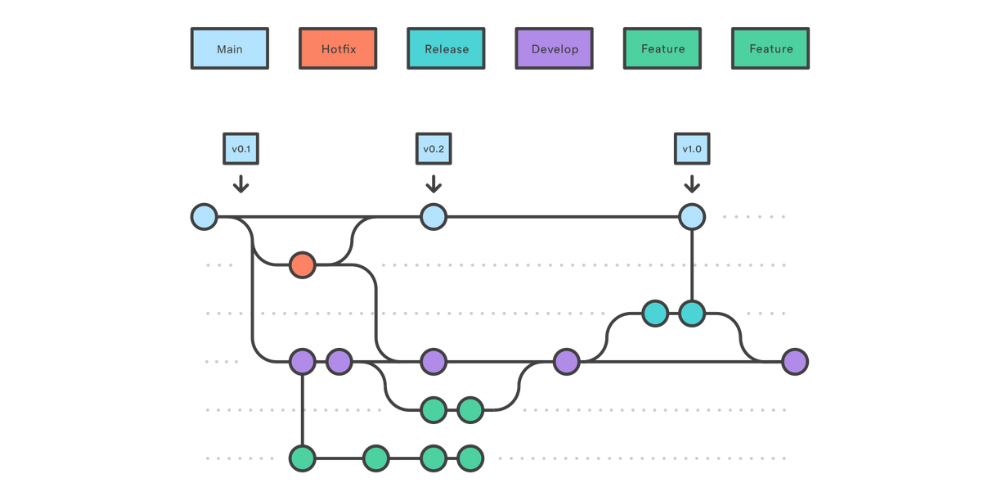
\includegraphics[width=\textwidth]{figures/impl/git-flow.png}
    \caption{příklad Gitflow workflow}
    \label{fig:gitflow}
\end{figure}



Ovšem například u repozitáře TTS-Thesis kde byly všechny naše práce jsme používali Trunk-Based Vývoj, neboli všechny akce se prováděli na hlavní větvi. Tento styl fungoval hlavně díky tomu že každý měl svou vlastní složku a není zde kód který by měl fungovat. Díky tomu jsme mohli mít instatntní nasazení vytvořeného PDF z \LaTeX ~souborů.

\section{Databáze}\label{sec:database}
Návrh probíhal jako první od vytvoření návrhu databáze. Na návrhu se podíleli všichni členové týmu \figureref{fig:job_distribution} jelikož bylo nutné aby všichni členové věděli co a jak bude v databázi strukturované. Návrh probíhal za pomocí placeného nástroje \textit{dbdiagram.io} kde se mohli všichni podílet i online na návrhu v jeden časový moment. Tento nástroj taktéž podporuje export do řady SQL dialektů, mimo jiné i do MySQL který jsme použili protože databáze MariaDB má stejnou syntaxi jako MySQL \sectionref{sec:data_storage}. 

V kompletním ER diagramu databáze \figureref{fig:dix:database_schema} lze vidět jednotlivé rozdělení tabulek dle barvy do jednotlivých logických celků \figureref{fig:database_schema:block}[, zjedodušené blokové schéma] . Každá tabulka má v prvním sloupci zda se jedná o klíč či ne, v druhém název atributu a v třetím jeho datový typ. Z jednotlivých řádků může být vidět závislost na ostatních tabulkách.

\begin{figure}[h]
    \centering
    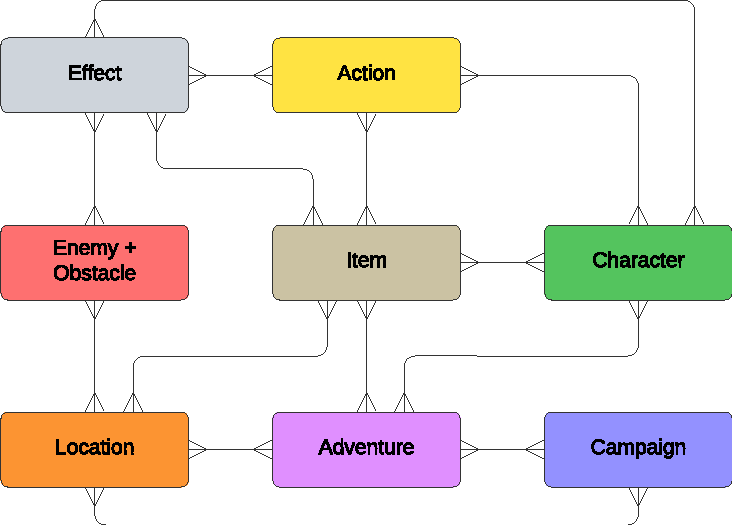
\includegraphics[width=0.5\textwidth]{../../shared/diagrams/er_macro.pdf}
    \caption{Zjednodušená databázové schéma podle logických celků}
    \label{fig:database_schema:block}
\end{figure}

Jako první je žlutá sekce která pojednává o \textbf{Akcích}. Základem je tabulka Action, která poté specifikuje o jakou akci se jedná, zda o \textit{útok, pohyb, dovednost, obnovení karet} nebo o \textit{přivolání poskoka}. Akce samozřejmě může mít i více specifikací o jakou kartu se jedná, poté skoro každý typ akce může mít nějaký přídavný efekt.

Šedá sekce \textbf{Efekt} přidává spoustu modifikací ať už jakékoli postavě jako například rezistenci na otrávení, nebo přidá modifikaci k útoku jako třeba \textit{krvácení}.

Zelená sekce se stará o \textbf{Postavu hráče}. Jako hlavní tabulka je zde \textit{Character} která má vazbu na definici o jakou postavu se bude jednat neboli tabulky \textit{Třída} a \textit{Rasa} a podle nich dostane své \textit{Akce}. Hráč má i inventář ve kterém může mít jednotlivé předměty které mu přidávají ať už statické bonusy tak jednorázové v boji.

Béžová sekce \textbf{Předmět} má na starosti \textit{předměty} a v jakých obchodech se nacházejí. Předměty jak již bylo zmíněno výše přidávají hráči bonusy.

\textbf{Protivník a Překážka} jsou v řervené sekci a specifikují protivníka nebo překážku v lokaci, ve které se bude bojovat. Jsou spojeny stejnou barvou protože tyto dvě entity jsou si velice podobné, jen jedna je statická a druhá dynamická.

Sekce \textbf{Lokace}, která je oranžová, specifikuje lokaci na které bude probíhat bojová interakce. Základem je tabulka \textit{Location} která má relace na vstupní a výstupní hexagony, na protivníky a překážky , dveře a na části lokace ze kterých se tato lokace skládá. 

A jako poslední sekce \textbf{Kampaň a Dobrodružství}, ikdyž jsou každá jinou barvou (Kampaň modrá a Dobrodružství fialová) tak spolu úzce souvisí. \textit{Kampaň} má příběh k dané lokaci, seznam \textit{dobrodružství} a seznam po jakých lokacích lze jít. \textit{Dobrodružství} má seznam hráčů kteří se účastní a  seznam dostupných lokací




